\documentclass[11pt]{article}
\usepackage{lmodern,setspace,amsmath,amssymb,amsfonts,amsthm,graphicx,multicol,grffile,float}
\usepackage{mathtools}
\usepackage{authblk,url,csvsimple,cuted,dblfloatfix,parskip}
\usepackage[a4paper, top=0.9in, bottom=1.05in, left=1.01in, right=1.01in]{geometry}
\usepackage[polish]{babel}
\usepackage[utf8]{inputenc}
\usepackage[unicode]{hyperref}
\usepackage{listings}
\usepackage{booktabs}
\usepackage{wrapfig}

\usepackage[linesnumbered,ruled,vlined]{algorithm2e}
\DontPrintSemicolon
\SetKw{Break}{break}
\SetKw{Continue}{continue}
\DeclareMathOperator*{\argmax}{arg\!max}
\DeclareMathOperator*{\argmin}{arg\!min}

\title{PTSZ - Zadanie 3 - Problem $F3 | | D_w$}
\author{Dariusz Max Adamski 136674 (grupa I9, godzina 8:15)}
\affil{dariusz.adamski@student.put.poznan.pl}
\date{Data oddania: \today}

\def\code#1{\texttt{#1}}

\begin{document}

\maketitle

\section*{Wstęp}

W tym sprawozdaniu opisane jest podejście rozwiązujące problem szeregowania zadań na trzech maszynach w systemie przepływowym z minimalizacją średniego ważonego opóźnienia.

\section{Generator instancji}

\begin{algorithm}
\caption{Algorytm generatora instancji dla problemu}
$t \coloneqq 0$ \;
\For{j \in 1 \dots n}{
    $\forall_{m \in \{1, 2, 3\}} \ldotp p_{j,m} \coloneqq \lfloor \text{Uniform}(1, 30) \rfloor$ \;
    $w_j \coloneqq \lfloor 100 * \text{Beta}(\alpha = 1.2, \beta = 2.3) \rfloor + 1$ \;
    $d_j \coloneqq t$ \;
    $t \coloneqq t + \lfloor \text{Uniform}(1, 20) \rfloor$ \;
}
Potasuj losowo zadania
\end{algorithm}

\begin{figure}[b]
\caption{Wizualizacja rozkładu wag zadań.}
\label{fig:weights}
\centering
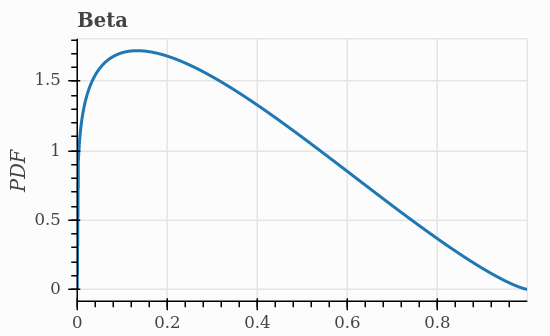
\includegraphics[scale=0.4]{beta.png}
\end{figure}

\subsection{Opis algorytmu}

Funkcja generująca instancje działa na zasadzie symulacji śledzącej aktualny czas $t$. Generowane jest $n$ zadań z czasem przetwarzania j-tego zadania na m-tej maszynie $p_{j,m}$, oczekiwanym czasem zakończenia $d_j$ i wagą zadania $w_j$. Czas przetwarzania na każdej maszynie jest losowany z rozkładu jednostajnego z minimalną wartością 1 i maksymalną 30. Jako oczekiwany czas zakończenia, algorytm przyjmuje aktualny czas symulacji $t$.

Waga zadania $w_j$ jest losowana z rozkładu Beta z parametrem $\alpha$ równym 1.2 i $\beta$ równym 2.3; rozkład jest przedstawiony na rysunku \ref{fig:weights}. Po wylosowaniu wagi ze wspomnianego rozkładu, ta jest mnożona razy 100, zaokrąglana w dół, a następnie dodawane jest do niej 1 -- dzięki temu wagi mają zakres $[1,101]$. Parametry rozkładu zostały dobrane tak, aby większość zadań miała małą wagę około 15, ale żeby ,,niespodziewanie'' pojawiały się też zadania z wagą około 90.

Po wygenerowaniu każdego zadania, czas symulacji $t$ jest zwiększany o krok losowany ze zdyskretyzowanego rozkładu jednostajnego z minimalną wartością 1 i maksymalną 20. Po wygenerowaniu wszystkich zadań, zadania są losowo tasowane.

\section{Algorytm szeregowania}

\begin{algorithm}
\caption{Algorytm dla problemu szeregowania}
$\forall_{m \in M}  t_m \coloneqq 0$ \;
\While{T \neq \varnothing}{
$j \coloneqq T[ \argmax_i h(T_i) ]$ \;
$t_1 \coloneqq t_1 + p_{j,1}$ \;
$t_2 \coloneqq \max \{ t_1, t_2 \} + p_{j,2}$ \;
$t_3 \coloneqq \max \{ t_2, t_3 \} + p_{j,3}$ \;
Zaplanuj zadanie $j$ \;
$T \coloneqq T \setminus \{ T_j \}$ \;
}
\end{algorithm}

\begin{algorithm}
\caption{Heurystyka $h(j)$ dla problemu szeregowania.}
$t_1' \coloneqq t_1 + p_{j,1}$ \;
$t_2' \coloneqq \max \{ t_1', t_2 \} + p_{j,2}$ \;
$t_3' \coloneqq \max \{ t_2', t_3 \} + p_{j,3}$ \;
$C_j \coloneqq t_3'$ \;
\Return $(d_j - C_j)^\alpha * w_j^\beta$
\end{algorithm}


\subsection{Oznaczenia}

Zbiór $T$ początkowo zawiera wszystkie zadania $T_1 \dots T_n$. Gdy zadanie jest dodane do uszeregowania, usuwane jest z tego zbioru.
Zbiór $M$ zawiera numery maszyn od 1 do 3.
Zmienne $t_m$ oznaczają aktualny czas symulacji na m-tej maszynie.

\subsection{Opis algorytmu}

Algorytm szeregowania działa w następujący sposób. Dla danego punktu w czasie symulacji $t_m$ wybierane jest najlepsze według heurystyki $h(j)$ zadanie ze zbioru kandydatów $T$. Rozpatrywane są tylko zadania, które nie zostały jeszcze dodane do uszeregowania.

Po wybraniu zadania $j$ obliczany jest po kolei czas maszyn $t_1$, $t_2$ i $t_3$. Później zadanie jest dodane do uszeregowania, a następnie jest usuwane ze zbioru kandydatów $T$.

Heurystyka $h(j)$ priorytetyzuje zadania z największą wagą $w_j$ i największym spóźnieniem $C_j - d_j$. Zarówno waga jak i spóźnienie są sparametryzowane parametrami $\alpha$ i $\beta$. Parametry są dopasowywane do instancji losowym przeszukiwaniem zakresu $[0.1, 10]$. Najlepsze parametry ustalane są przez uruchomienie algorytmu 20 razy. Tylko najlepszy wynik szeregowania jest zapisywany.


\subsection{Analiza złożoności}

Złożoność algorytmu to $O(n^2)$, gdzie $n$ to wielkość instacji - liczba zadań. Złożoność wynika z tego, że zachłannie planujemy $n$ zadań, a przy planowaniu każdego zadania wykonujemy operację argmax na zbiorze kandydatów $T$, która wykonuje się w maksymalnie $n$ krokach. Wynika z tego, że złożoność wynosi $O(n*n)$, czyli $O(n^2)$. Kilkukrotne wywołanie algorytmu z różnymi parametryzacjami heurystyki nie wpływa na złożoność.

\end{document}
